\documentclass[11pt,a4paper]{article}
\usepackage[spanish]{babel}
\usepackage[utf8]{inputenc}
\usepackage[top=2cm, bottom=2cm, left=2cm, right=2cm]{geometry}
\usepackage{commath,amsmath,lastpage,float,sectsty,hyperref,graphicx,pdfpages,fancyhdr,listings,siunitx,gensymb}

\sectionfont{\fontsize{12}{15}\selectfont}
\linespread{1.25} % Interlineado 1.5
\renewcommand{\rmdefault}{phv} % Arial
\renewcommand{\sfdefault}{phv} % Arial

\hypersetup{
    pdftitle={Trabajo Práctico 2},
	pdfsubject={Análisis Numérico I},
	pdfauthor={Kristal Juan Ignacio},
}

\lstset{
  basicstyle=\ttfamily,
  columns=fullflexible,
  frame=single,
  breaklines=true,
  literate={°}{{$\degree$}}1,
  postbreak=\mbox{\textcolor{red}{$\hookrightarrow$}\space},
}

\fancypagestyle{enunciado}{
    \fancyhf{}
    \fancyhead[C]{Enunciado provisto por la catedra}
}

\pagestyle{fancy}
\fancyhf{}
\fancyhead[R]{Trabajo Práctico 2 - 2018c2}
\fancyhead[L]{75.12 Análisis Numérico I}
\renewcommand{\headrulewidth}{0.4pt}
\fancyfoot[L]{9779}
\fancyfoot[R]{\thepage de \pageref*{LastPage}}
\renewcommand{\footrulewidth}{0.4pt}
\setlength{\footskip}{17pt}

\fancypagestyle{onlyheader}{
\fancyfoot{}
}

\begin{document}

\begin{titlepage}
	\hfill
\includegraphics[width=6cm]{figuras/fiuba.jpg}
    \begin{center}
    \vfill
    \Huge \textbf{Trabajo Práctico 2}
    \vskip2cm
    \Large [75.12] Análisis Numérico I\\
    Segundo cuatrimestre de 2018
    \vfill
    \begin{tabular}{|l|c|r|}
	\hline
	Alumno & Padrón & Mail\\
	\hline
	\hline
	Kristal, Juan Ignacio & 99779 & kristaljuanignacio@gmail.com\\
	\hline
	\end{tabular}
    \vskip2cm
    \end{center}

    Curso 07:

    \begin{itemize}
    \item Dr Daniel Fabian Rodriguez
    \item Valeria Machiunas
    \item Federico Balzarotti
    \item Michael Portocarrero
    \end{itemize}

\end{titlepage}

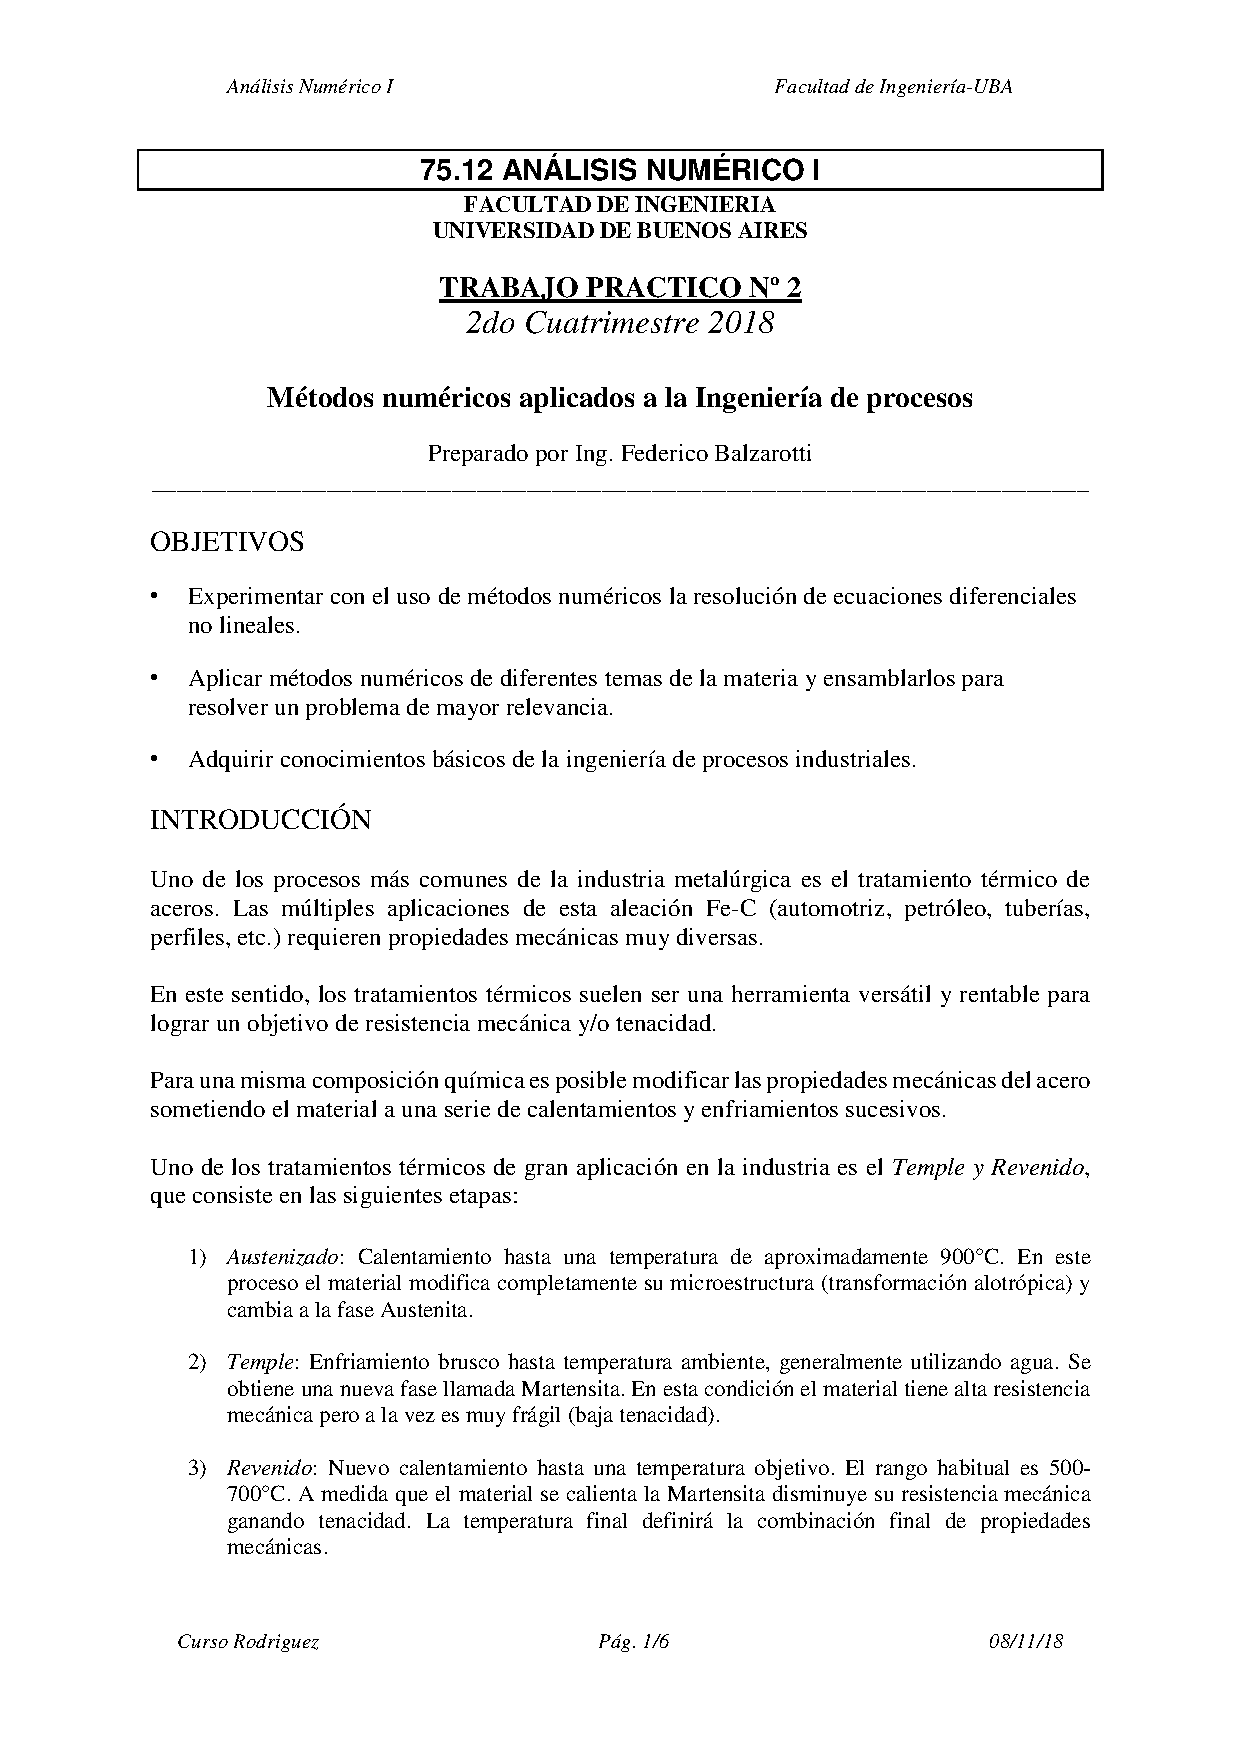
\includepdf[pages=-,pagecommand={\thispagestyle{enunciado}}]{TP2-Enunciado.pdf}

\pagenumbering{gobble}
\tableofcontents
\thispagestyle{onlyheader}
\newpage

\pagenumbering{arabic}
\setcounter{page}{1}

\section{Introducción}
El trabajo práctico tiene como objetivo la resolucion de ecuaciones diferenciales mediante distintos metodos y la comparacion de los mismos asi como la resolucion de sistemas de ecuaciones no lineales. Para ello, se utilizara un modelo para el tratamiento termico de tubos de acero mediante la ley de la conservacion de la energia. La siguiente es la ecuacion diferencial a resolver:

\begin{equation}
-mC \frac{dT}{dt} = h_c S (T - T_\infty) + \sigma \epsilon (T^4 - T^4_\infty)
\end{equation}

Específicamente:

\begin{itemize}
\item Se estimarán los valores de temperatura (por conveccion y radiacion) a lo largo del tiempo.
\item Se determinará que algoritmo resulta ser mas exacto.
\item Se obtendra una temperatura de soaking y un tiempo de soaking para el proceso.
\item Se variará la temperatura del horno de trata en diferentes sectores para alcanzar valores deseados de soaking.
\item Se automatizará dicho proceso mediante la resolucion de un SENL.
\end{itemize}

\section{Desarrollo}

\subsection{Calculo de temperatura}

Para los cálculos de temperatura se utilizaron dos metodos de resolucion de ecuaciones diferenciales. El metodo de Euler y el metodo de Runge-Kutta de cuarto orden (a partir de ahora, RK4). Se utilizo el algoritmo del libro de Hernan Gonzales \cite{Gonzales}. Dicho calculo fue dividido en dos partes, la temperatura generada por el proceso de conveccion y la del proceso de radiacion.

\subsection{Proceso de conveccion}

El proceso de conveccion estaba dado por una ecuacion diferencial de variables separables por lo que su resolucion matematica era posible y sencilla. De este modo se lograron calcular estimaciones de dicha funcion con ambos metodos y se observa una comparacion con los valores exactos. Con la informacion exacta es posible determinar el error relativo de ambos metodos en base a dichos valores.

El grafico la función exacta y los valores calculados numericamente de ambos metodos pueden observarse en la figura \ref{fig:metodos}

Usando la formula del calculo de errores relativos fue sencillo obtener el error de cada metodo en cada valor de tiempo particular. En la figura \ref{fig:errores} se puede observar un grafico comparativo en escala logaritmica para una mejor apreciacion. En dicho grafico se observa claramente que el metodo de RK4 tiene un error menor y por lo tanto es el metodo que se usará para el proximo calculo. Esperable dado que el orden de error de RK4 es mayor.

\subsection{Proceso de conveccion y radiacion}

Con RK4 determinado como el algoritmo más exacto se resolvera mediante dicho metodo la ecuacion diferencial completa. En este caso no hay una función exacta para comparar y observar el error pero determinamos que RK4 es mas preciso que Euler.

A modo de comparación se usará la función calculada previamente con unicamente la conveccion y se observa que el intercambio por radiacion es claramente significativo en la figura \ref{fig:comp}

\subsection{Temperatura y tiempo de soaking}

Dado que tanto la temperatura como el tiempo de soaking son valores muy importantes para este proceso fueron calculados para los valores iniciales de temperatura. Con el horno a temperatura constante a 696 \degree C. Para obtener este valor de tiempo se busco el punto donde la temperatura alcanzada es de 10 \degree C menor a la final. Para alcanzar la temperatura de soaking se busco el promedio de temperatura durante ese intervalo de tiempo.

Luego se variaron las temperaturas para alcanzar un tiempo de soaking menor. Con el tiempo de soaking a 10 minutos fijo, se variaron las temperaturas manualmente hasta llegar a dicho tiempo y luego se planteo un sistema de ecuaciones no lineales el cual fue resuelto con el metodo de punto fijo para obtener un resultado más preciso. Se utilizaron 2 cifras decimales como condicion de corte pues el problema, por algun motivo desconocido, no lograba a conseguir errores menores para valores de temperatura menores a los 800  \degree C.

\begin{figure}[H]
	\makebox[\textwidth][c]{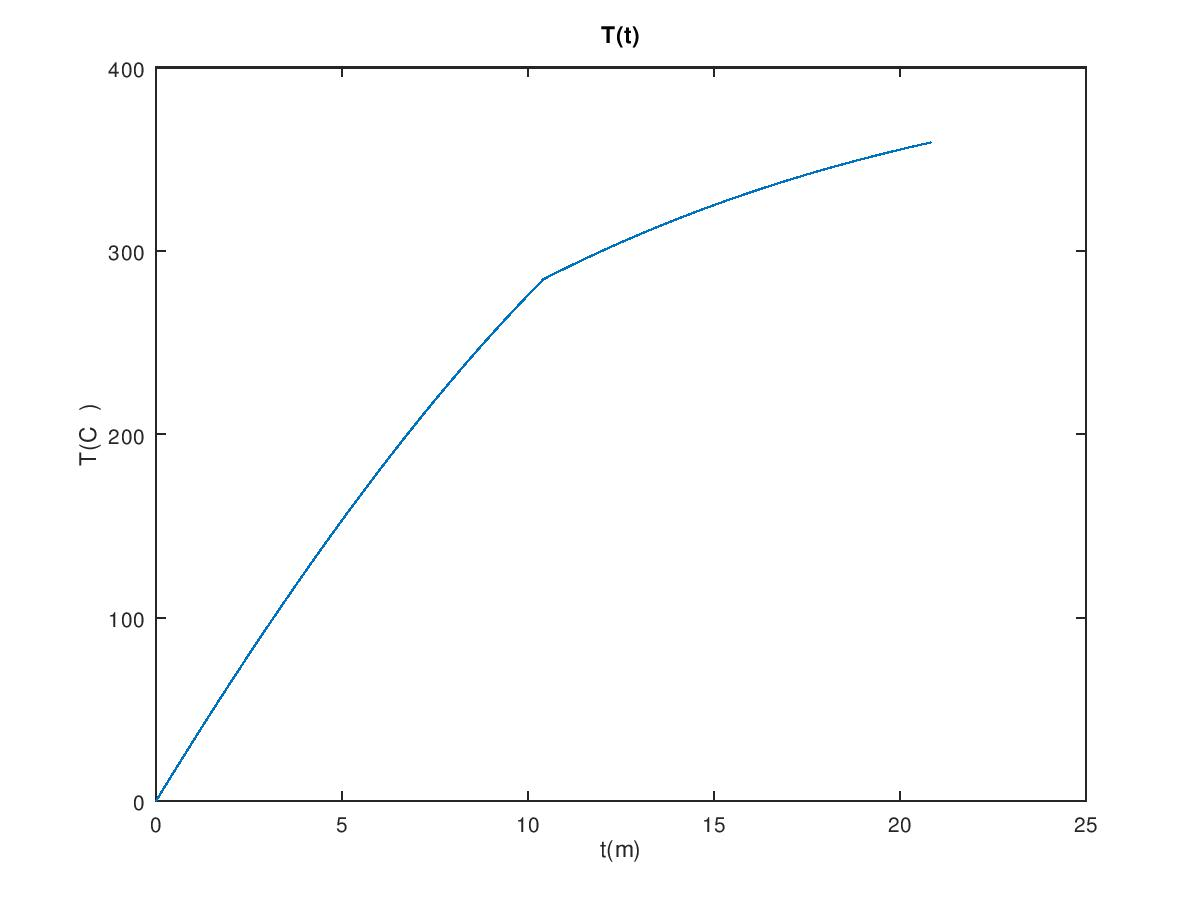
\includegraphics[width=1.2\textwidth]{figuras/A.jpg}}
	\caption{Evolución de 696\degree C}
    \label{fig:A}
\end{figure}

\begin{figure}[H]
	\makebox[\textwidth][c]{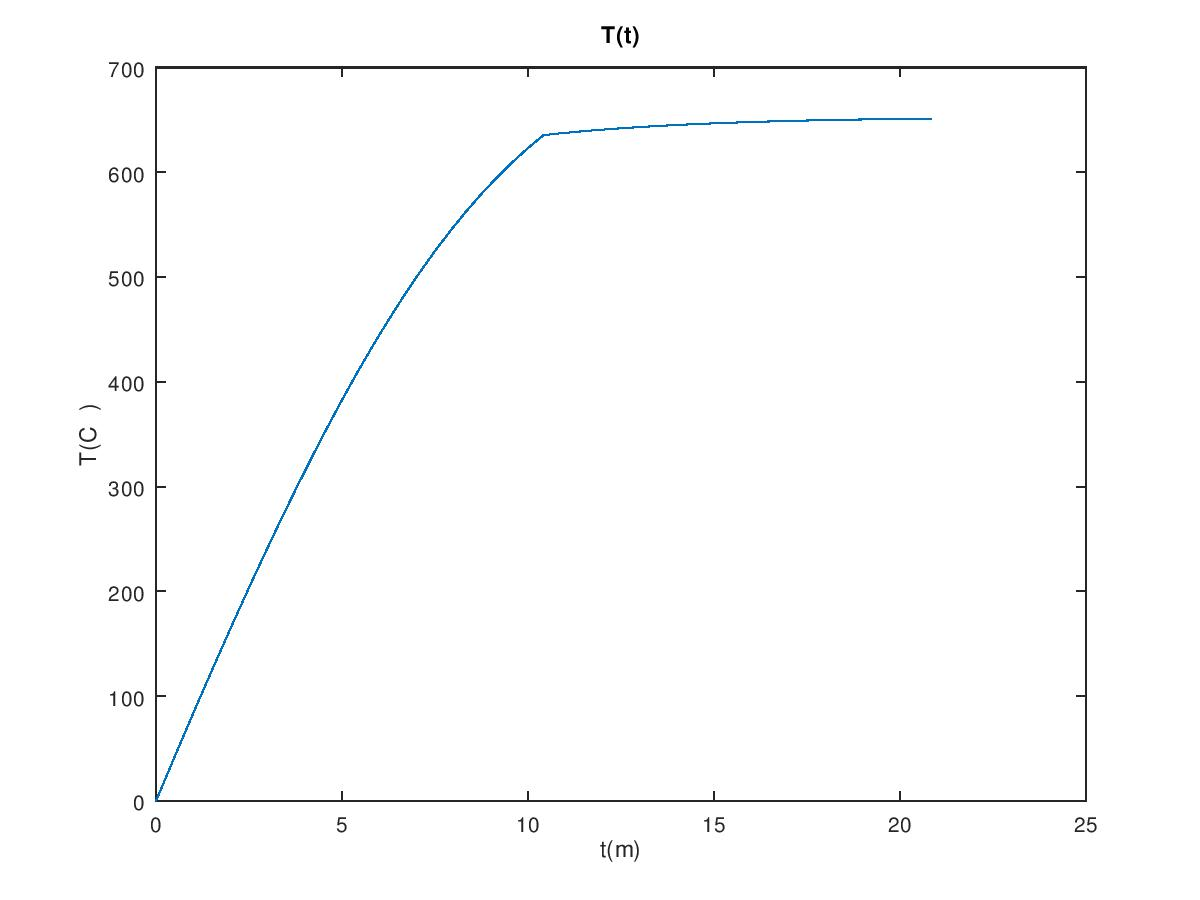
\includegraphics[width=1.2\textwidth]{figuras/B.jpg}}
	\caption{Evolución de 648\degree C}
    \label{fig:B}
\end{figure}

\begin{figure}[H]
	\makebox[\textwidth][c]{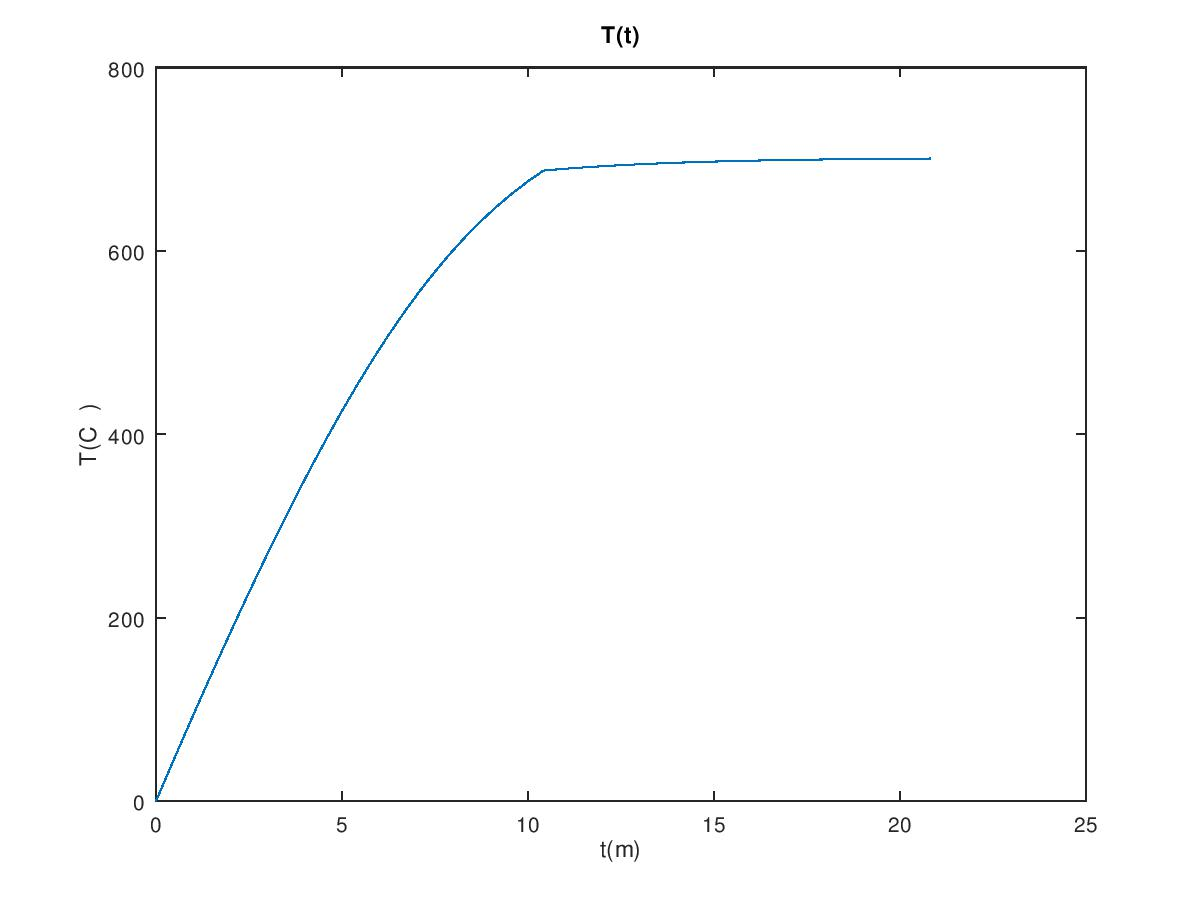
\includegraphics[width=1.2\textwidth]{figuras/C.jpg}}
    \caption{Evolución de 698\degree C}
	\label{fig:C}
\end{figure}

Finalmente se tomaron 3 temperaturas (696 \degree C, 648 \degree C y 698 \degree C) y se resolvio el sistema, graficando la evolucion de la temperatura en las figuras \ref{fig:A}, \ref{fig:B} y \ref{fig:C} respectivamente.

\section{Resultados}

\subsection{Graficos comparativos y evolucion de la temperatura respecto al tiempo}

Utilizando ambos metodos de resolucion de ecuaciones diferenciales se llegaron a los siguientes resultados para calor por conveccion unicamente:

\begin{figure}[H]
	\makebox[\textwidth][c]{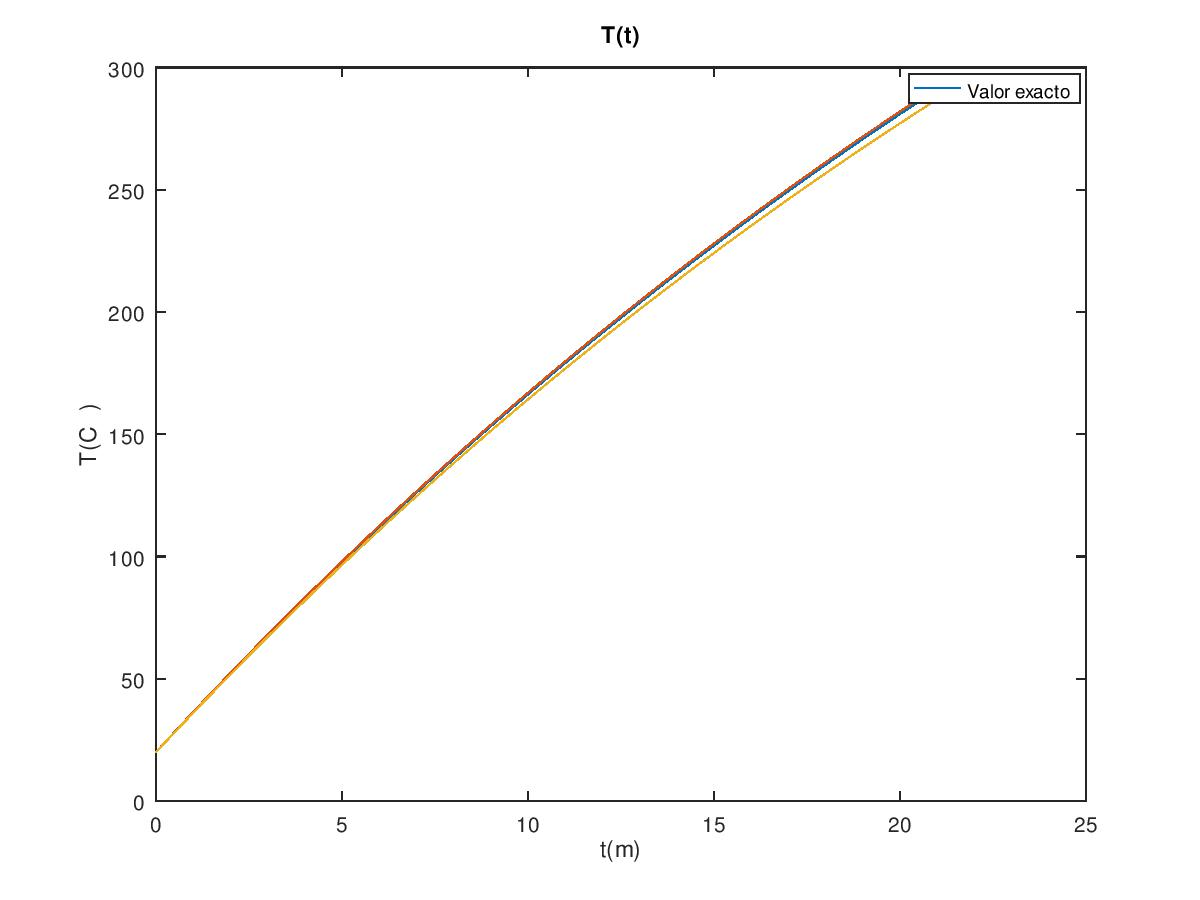
\includegraphics[width=1.2\textwidth]{figuras/metodos.jpg}}
	\caption{Métodos}
	\label{fig:metodos}
\end{figure}

\begin{figure}[H]
	\makebox[\textwidth][c]{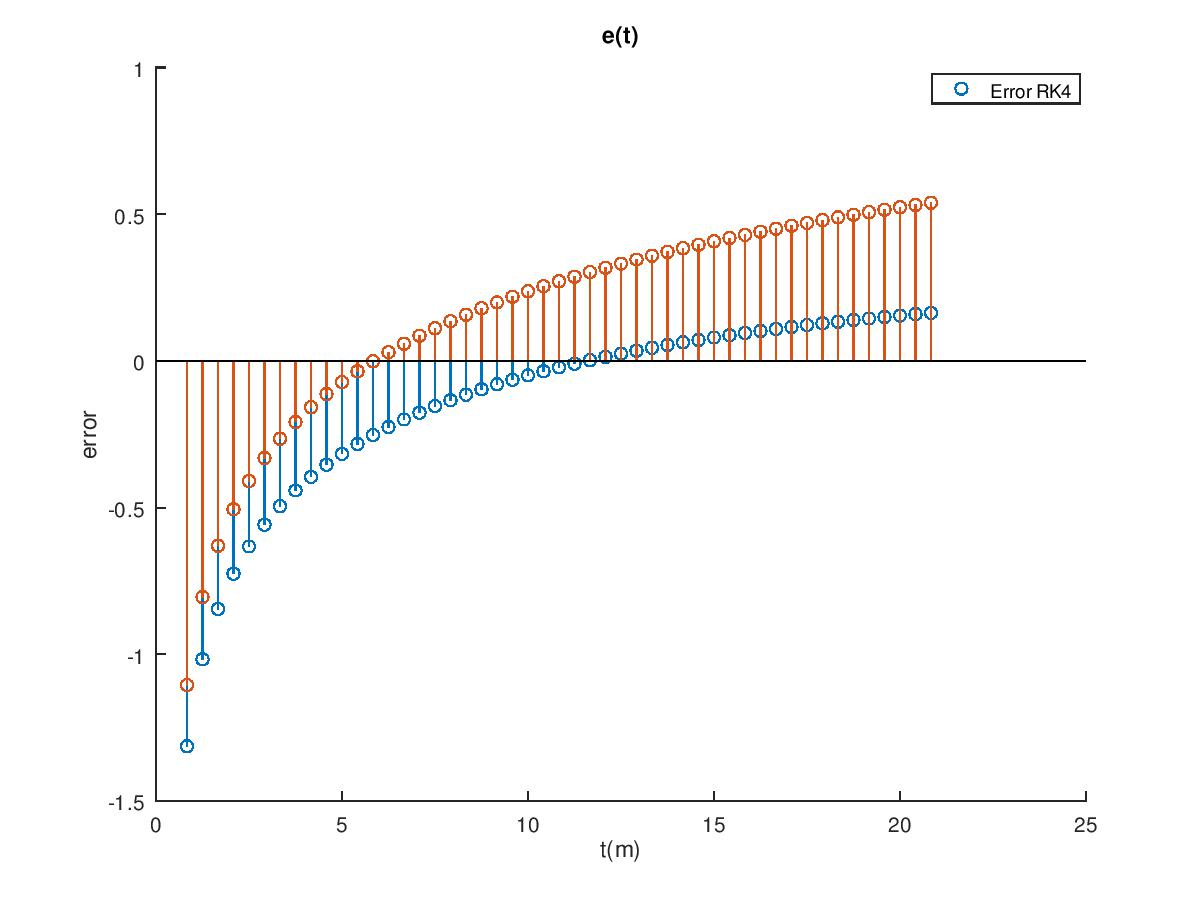
\includegraphics[width=1.2\textwidth]{figuras/errores.jpg}}
	\caption{Errores}
	\label{fig:errores}
\end{figure}

Utilizando el metodo de RK4 se llego a la siguiente grafica comparativa para el calor por conveccion y radiacion:

\begin{figure}[H]
	\makebox[\textwidth][c]{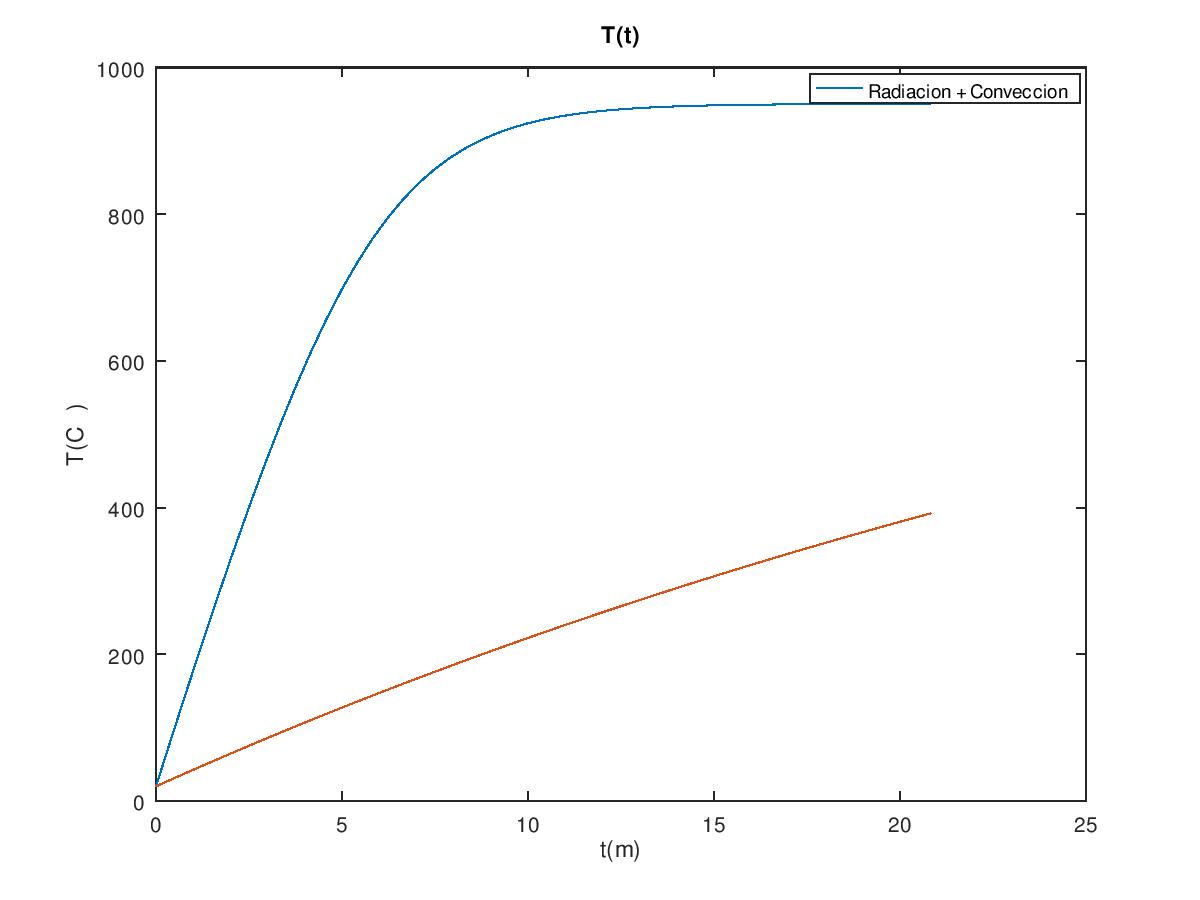
\includegraphics[width=1.2\textwidth]{figuras/comparacion.jpg}}
	\caption{Comparación}
	\label{fig:comp}
\end{figure}

Se obtuvieron:

tiempo\_soaking =  2.0833
temp\_soaking =  667.45

Y mediante el tanteo se aumento el tiempo de soaking a 10 minutos con los valores de temperatura:

T1 = 780
T2 = 680

Finalmente la tabla final de valores con el SENL:

\begin{table}[!h]
\centering
\begin{tabular}{|l|l|l|l|l|l|}
\hline
Caso & sk & Tsk & T1 & T2 & Iteraciones\\
\hline
A & 10min & 667\degree C & 777.41\degree C & 684.22\degree C & 13 \\
B & 10min & 648\degree C & 758.84\degree C & 665.49\degree C & 13 \\
C & 10min & 698\degree C & 792.59\degree C & 714.23\degree C & 13 \\
\hline
\end{tabular}
\end{table}

\section{Conclusiones}

Las ecuaciones diferenciales resueltas por metodos numericos si bien tienen su grado de error pueden solucionar problemas incalculables. Esto es extremadamente util para casos como este donde hay ecuaciones que no son resolvibles pero un pequeño grado de error no es lo suficientemente significativo entonces los metodos como Euler o RK4 pueden optimizar el tiempo requerido para el calculo y resolucion de un problema. Se pudo observar que RK4 es un algoritmo con mayor precision pero tambien un algoritmo de mayor complejidad que Euler. En la teoria, como RK4 es un algoritmo de orden mayor de error que Euler era esperable que su precision fuese mayor. Resulta extraño que el metodo de punto fijo no haya podido converger pero haya logrado dar una precision aceptable. La condicion de corte del metodo fue reducida a una cifra decimal menos debido a esto y logro converger en todos los casos propuestos.

Hablando mas especificamente respecto de este trabajo practico se puede concluir en que el calor por radiacion no es para nada despreciable en comparacion al de conveccion como fue observado graficamente.

Los metodos numericos son extremadamente utiles para cuando existen ecuaciones diferenciales no lineales pues son mucho mas faciles de resolver y con errores pequeños. Para las ecuaciones diferenciales lineales el error cometido puede incluso ser lo suficientemente pequeño pero teniendo la solucion exacta en general sería mejor obtener dicho valor siempre y cuando no sea demasiado costoso.

En tanto a los metodos de resolucion para SENL es evidente que es mucho más sencillo resolverlos con dichos metodos si existen multiples variables. Se pudo observar en el item 3 del trabajo practico durante el tanteo que a mi particularmente me tomo al menos unos 15 intentos hasta llegar a un resultado que siquiera llega a la precision del metodo de punto fijo. La cantidad de iteraciones del metodo para los 3 casos fueron siempre 13, no solo es mas rapido sino que tambien mas preciso. Para este tipo de problemas inversos resulta ser muy util.

Se podría aumentar la cantidad de iteraciones del metodo de punto fijo para obtener un error aun menor y acercarse aun más a la realidad, pero la relacion con respecto a su costo puede no ser rentable. La velocidad de convergencia de punto fijo puede ser lo suficientemente costosa como para optar por una menor precision con una menor cantidad de recursos.

\newpage
\appendix
\section{Anexo I: Código Fuente}

El programa utilizado es GNU Octave, versión 4.2.2 y se procuró utilizar sintaxis compatible con Matlab, teniendo como única excepción la función \texttt{fplot} que brinda Octave para graficar funciones, despues de consultar con los docentes.


\newpage
\lstinputlisting[language=Octave,title=\texttt{main.m}]{src/main.m}

\newpage
\section{Anexo II: Resultados Numéricos}


\phantomsection 
\addcontentsline{toc}{section}{Bibliografía}
\renewcommand\refname{Bibliografía}
\begin{thebibliography}{9}

\bibitem{Gonzales} 
Gonzales, Hernan: 
\textit{Análisis Numérico, Primer Curso}
Buenos Aires: Nueva Librería, 2002.

\end{thebibliography}
\end{document}